\chapter{На каких языках программирования пишутся операционные системы}
\label{ch:operating-sysmets}

В главе исследуется объект Викиданных <<операционная система>> (operating system) и его свойства. 
Построен список операционных систем (ОС), включающий информацию о~их~<<предках>>\footnote{%
%
<<Предки>>~--- здесь операционные системы, послужившие основой для создания новых ОС.%
%
}, 
времени создания, языках программирования, на которых написаны ОС. 
Также построена гистограмма, показывающая количество программ, 
написанных на том или ином языке программирования с~указанием операционной системы. 
У большого количества ОС в Викиданных не указан язык программирования, 
на котором она разрабатывалась, а именно: 
на 2020 год это свойство указано лишь у~29\,\% из общего количества систем. 
Викиданные стремительно пополняются новой информацией, что особенно отрадно, 
поскольку они играют большую роль в документировании программного обеспечения.



\section{Список операционных систем}
С помощью запроса~\ref{lst:all_operating_systems} получим список всех операционных систем.
%\begin{marginfigure}[-11\baselineskip]
\begin{lstlisting}[ language=SPARQL, 
                caption={\href{https://w.wiki/n89}{Список всех операционных систем}\protect\footnotemark},
                numbers=none,
                label=lst:all_operating_systems
	            ]
SELECT ?os ?osLabel WHERE
{
    ?os wdt:P31 wd:Q9135. # instance of operating system
    SERVICE wikibase:label { bd:serviceParam wikibase:language "ru, en"}
}
\end{lstlisting}
\footnotetext{Получено: 510 операционных систем в 2017 году и 1086 систем в~2020 году. Ссылка на~SPARQL-запрос: \href{https://w.wiki/n89}{https://w.wiki/n89}.}
%\end{marginfigure}


Наиболее полными и проработанными операционными системами в~Викиданных на~2021 год были 
\wdqName{Microsoft Windows}{1406}, 
\wdqName{Windows 8}{5046}, 
\wdqName{GNU}{44571}, 
\wdqName{Windows 10}{18168774}, имеющие по~24 заполненных свойства. % \autocite{prowd_os_link}.
Почти пустыми и малоинформативными операционными системами на~2021 год были: 
\wdqName{MagiC}{1884068}, \wdqName{KallistiOS}{1722492}, \wdqName{Novell DOS}{3345389} и ряд других. 
У~этих систем было заполнено лишь одно свойство. % \autocite{prowd_os_link}.
%
По данным ProWD, у единственной в Викиданных отечественной ОС 
\wdqName{Miraculix}{4044344} заполнено 10 свойств. % \autocite{prowd_os_link_ru}.




\section{Предшественники операционных систем и даты выпуска}

Запрос~\ref{lst:base_of_operating_systems} позволяет получить 
список \href{https://www.wikidata.org/wiki/Property_talk:P144}{базовых (P144)} операционных систем. 
Этот запрос показывает соответствие 
между \wdqName{операционной системой}{9135} и её <<предком>>, 
то есть предшествующей операционной системой, на которой она основана.

\marginnote[3\baselineskip]{
    \MarginQuestion
	На основе какой из операционных систем~--- 
	\href{https://w.wiki/n8U}{Debian}, 
	\href{https://w.wiki/n8V}{Android}, 
	\href{https://w.wiki/n8W}{Ubuntu}, 
	\href{https://w.wiki/n8X}{ядро Linux}~---  
	было создано больше всего других операционных систем?

	См. ответ %~\ref{answer:os_base} 
    на с.~\pageref{answer:os_base}.
}

\begin{lstlisting}[ language=SPARQL, 
                caption={\href{https://w.wiki/5CKF}{Список базовых операционных систем}\protect\footnotemark},
                numbers=none,
                label=lst:base_of_operating_systems
                ]
SELECT ?os ?osLabel ?base ?baseLabel WHERE
{
    ?os wdt:P31 wd:Q9135;   # is instance of operating system
        wdt:P144 ?base.     # is based on ?base
    SERVICE wikibase:label { bd:serviceParam wikibase:language "ru, en" }
}
\end{lstlisting}
\footnotetext{Получено: 47 базовых операционных систем в 2017 году и 118 систем в~2020 году. 
Ссылка на~SPARQL-запрос: \href{https://w.wiki/5CKF}{https://w.wiki/5CKF}.}




%\section{Дата выпуска операционных систем}

Список операционных систем с указанием даты их создания 
получим с помощью запроса~\ref{lst:inception_time_of_operating_systems}.
%
\marginnote[3\baselineskip]{%
    \MarginQuestion
    Какую из операционных систем~--- 
    \href{https://w.wiki/n8P}{Newton OS}, 
    \href{https://w.wiki/n8Q}{Ubuntu Touch} или 
    \href{https://w.wiki/n8R}{JavaOS}~--- 
    разработала компания \href{https://w.wiki/n8S}{Apple}?

    См. ответ %~\ref{answer:what_system_created} 
    на с.~\pageref{answer:what_system_created}.%
}

\index{SPARQL!YEAR}
\index{График!Timeline!hide}
\begin{lstlisting}[ language=SPARQL, 
	caption={\href{https://w.wiki/5CKS}{Список операционных систем с датой их создания}\protect\footnotemark},
	label=lst:inception_time_of_operating_systems,
    numbers=none,
    texcl=false,
	]
#defaultView:Timeline{"hide": "?when"}
SELECT DISTINCT ?os ?osLabel ?when (YEAR(?when) as ?date) ?pic WHERE
{
    ?os wdt:P31 wd:Q9135;           # instance of operating system
        wdt:P571 ?when.             # inception date
    OPTIONAL { ?os wdt:P18 ?pic }
    SERVICE wikibase:label {bd:serviceParam wikibase:language "ru, en"}
}
\end{lstlisting}
\footnotetext{Получено: 30 дат создания ОС в 2017 году и 238~дат в~2020 году. 
    Ссылка на SPARQL-запрос: \href{https://w.wiki/5CKS}{https://w.wiki/5CKS}.}


\newpage
\index{График!Timeline}
\index{График!Timeline!hide}
Команда \lstinline|#defaultView:Timeline| в строке~1 
запроса~\ref{lst:inception_time_of_operating_systems} 
похожа на комментарий, 
а~в~действительности является инструкцией для сервиса WDQS\footnote{%
    См. описание сервиса WDQS (Wikidata Query Service)~на~с.~\pageref{sect:WDQS}.%
    \index{Wikidata Query Service!Timeline}
}. 
Эта инструкция позволяет получить диаграмму на~рис.~\ref{fig:os_creation} 
в виде временной шкалы.

В этой строке 1 запроса~\ref{lst:inception_time_of_operating_systems} 
параметры \lstinline|{"hide": "?when"}| 
команды \lstinline|#defaultView:Timeline| позволяют скрыть вывод переменной \lstinline|?when|, 
оставив от даты только год (функция \lstinline|YEAR()|) 
и название ОС (переменная \lstinline|?osLabel|). 
Благодаря этому мы видим в центре рис.~\ref{fig:os_creation} 
под изображением смартфона \mbox{не ``1 January 1993''}, а~только ``1993''. 

Таким образом, результатом запроса~\ref{lst:inception_time_of_operating_systems} 
является временная шкала (англ. \textit{timeline}) создания (точнее, выпуска\sidenote[][-8pt]{%
%
Создание операционной системы~--- это длительный процесс, часто занимающий годы. 
Поэтому здесь указана дата первой версии системы. 
\newline
}%
) %
операционных систем (рис.~\ref{fig:os_creation}). 
Кроме временной шкалы, есть много других способов представления результатов запросов 
в графической форме, описанных в документации\sidenote{%  \autocite{WQSResultViews}
%
    См. справочную страницу на~сайте Викиданных 
    \index{Wikidata Query Service!Help/Result Views}
    \emph{Wikidata:SPARQL query ser\-vice/Wikidata Query Help/Result Views} 
    о~вариантах представления результатов SPARQL-запросов 
    по~ссылке: \href{https://www.wikidata.org/?curid=29285671}
                                        {https://www.wikidata.org/?curid=29285671}.%
%
}.\, Количество полученных результатов запроса~\ref{lst:inception_time_of_operating_systems} 
составляет только 238 операционных систем (то есть 22\,\% от всего количества ОС) на 2020 год. 
Связано это с тем, что у 78\,\% ОС поле <<дата создания>> не заполнено.

\begin{figure*}[h!]
	\includegraphics{./chapter/operating_system/os-creation.png}
    \caption[Часть временной шкалы с датами выпуска ОС.]{
        Часть временной шкалы с датами выпуска операционных систем\\с~1955 по~2020 год}%
    %Шкала построена по запросу~\protect\ref{lst:inception_time_of_operating_systems}.}
	\label{fig:os_creation}
\end{figure*}





\section{Количество операционных систем, написанных на языках программирования}

В листинге~\ref{lst:count_os_on_languages} представлен SPARQL-запрос для получения 
списка языков программирования с~выводом количества написанных на~них ОС.

\index{SPARQL!COUNT}
\index{SPARQL!ORDER BY!двойная сортировка}
\begin{lstlisting}[ language=SPARQL, 
	caption={\href{https://w.wiki/uat}
            {Список языков программирования и количество написанных на них\\операционных систем}\protect\footnotemark},
    numbers=none,
	label=lst:count_os_on_languages
	]
# Languages and number of OS written in these languages
SELECT ?lang ?langLabel (COUNT(*) AS ?countOS) WHERE 
{
	?os wdt:P31 wd:Q9135. # is instance of operating system
	?os wdt:P277 ?lang. # is written in programming language ?lang
    SERVICE wikibase:label {bd:serviceParam wikibase:language "ru, en"}
}
GROUP BY ?lang ?langLabel
ORDER BY DESC(?countOS) ASC(?langLabel)
\end{lstlisting}
\footnotetext{Получено: 24 языка программирования с количеством 
написанных на~них операционных систем в 2017 году 
и 36 языков в~2021 году. 
Ссылка на~SPARQL-запрос: \href{https://w.wiki/uat}{https://w.wiki/uat}.}



\newpage\phantom{blabla}
\newpage
%
\begin{marginfigure}[0\baselineskip]
    \includegraphics[width=6cm]{chapter/operating_system/prog_lang_os.png}
    \caption[Дерево языков программирования и написанных на них ОС.]{Дерево языков программирования и написанных на них операционных систем}
	\label{fig:prog_lang_os}%
\end{marginfigure}
%

\index{SPARQL!ORDER BY!двойная сортировка}
Команда \lstinline|ORDER BY DESC(?countOS) ASC(?langLabel)| в~запросе~\ref{lst:count_os_on_languages} 
используется для двойной сортировки значений в таблице. 
Все языки программирования в этой таблице сначала сортируются по~убыванию количества операционных систем, 
которые написаны на них. Затем, если для каких-либо языков это число совпадает, 
сортировка идёт по именам языков.

Результат SPARQL-запроса \ref{lst:count_os_on_languages} показывает, 
что преимущественно ОС пишут на языках Си (известно 46 операционных систем, написанных на языке Си) и ассемблер (42 ОС). 
На~третьем месте~--- язык C++ (16 ОС).



С помощью запроса~\ref{lst:lang_tree} можно получить диаграмму языков программирования 
и написанных на них операционных систем в виде дерева (рис.~\ref{fig:prog_lang_os}). 
В этом дереве каждая строчка~--- это язык программирования. 
По щелчку мыши можно развернуть язык и увидеть список операционных систем, 
написанных с использованием этого языка. 
Если язык или система имеют рисунок или логотип в~Викиданных, 
то они используются в качестве иконок.
\marginnote[1\baselineskip]{
    \MarginQuestion
    Сложное задание для самостоятельной работы. 
    Измените запрос~\ref{lst:lang_tree} (\href{https://w.wiki/ucB}{https://w.wiki/ucB}) так, 
    чтобы рядом с языком программирования было дано число операционных систем, написанных на этом языке.
}
%
\marginnote[2pt]{%
    \MarginQuestion
    Простое задание. 
    <<Переверните>> запрос~\ref{lst:lang_tree}, 
    то есть строчки верхнего уровня пусть содержат не языки программирования, 
    а операционные системы. 
    При <<разворачивании>> мы должны видеть список языков, на которых написана система.%
    \newline
}

\index{SPARQL!OPTIONAL}
\index{График!Tree}
\begin{lstlisting}[ language=SPARQL, 
	caption={\href{https://w.wiki/ucB}{Список языков программирования и написанных на них операционных систем}\protect\footnotemark},
    numbers=none,
	label=lst:lang_tree
	]
# Languages and operating systems written in these languages
#defaultView:Tree
SELECT ?lang ?image ?logoImage ?langLabel 
       ?os ?osImage ?osLogoImage ?osLabel 
WHERE 
{
	?os wdt:P31 wd:Q9135. # is instance of operating system
	?os wdt:P277 ?lang. # is written in programming language ?lang
	OPTIONAL { ?lang wdt:P18 ?image. }
	OPTIONAL { ?lang wdt:P154 ?logoImage. }
	OPTIONAL { ?os wdt:P18 ?osImage. }
	OPTIONAL { ?os wdt:P154 ?osLogoImage. }
    SERVICE wikibase:label {bd:serviceParam wikibase:language "ru, en"}
}
\end{lstlisting}
\footnotetext{Получено: 146 языков программирования с написанными на них операционными системами в 2021 году. Ссылка на SPARQL-запрос: \href{https://w.wiki/ucB}{https://w.wiki/ucB}.}
%








\newpage
\section{Полнота Викиданных по числу операционных систем}

По данным сайта \href{https://www.operating-system.org/}
                             {www.operating-system.org}, 
существует 613 операционных систем. 
Викиданные на~2017 год содержали информацию лишь о 510 операционных системах. 
Результаты запросов~\ref{lst:inception_time_of_operating_systems} 
                  и~\ref{lst:count_os_on_languages} показывают, 
что многие объекты ОС плохо заполнены, а то и вовсе практически пусты 
(например, у~систем \wdqName{Novell DOS}{3345389} и \wdqName{MagiC}{1884068} 
заполнено всего одно свойство).

В 2020 году Викиданные содержали информацию о 1086 операционных системах 
(запрос~\ref{lst:all_operating_systems}), что свидетельствует о значительных изменениях, 
а именно: за три года (с 2017 года) количество операционных систем более чем удвоилось: с 510 до 1086. 
Однако большое количество объектов по-прежнему плохо заполнены, 
например по результатам запроса \ref{lst:inception_time_of_operating_systems} 
информация о дате выпуска заполнена всего у 238 ОС. 
Из этого можно сделать вывод, что хотя Викиданные неполны, но они стремительно пополняются.




\section{Языки программирования, используемые для написания операционных систем}
%
\index{График!BarChart}
%\begin{figure}[h]
\begin{marginfigure}[0\baselineskip]
	\includegraphics{./chapter/operating_system/count-os-written-on-languages.png}
    \caption[Первые языки, на которых написано больше всего ОС, 2020 год.]{Первые восемь языков, на которых написано больше всего операционных систем, 2020 год}
	\label{fig:count-os-written-on-languages}
\end{marginfigure}

Если взглянуть на количество операционных систем, для которых указано свойство <<язык программирования>>, 
    то можно увидеть, что это свойство заполнено лишь у 116 из 1086 объектов. 
    По~данным на 2020 год (рис.~\ref{fig:count-os-written-on-languages}), 
    больше всего операционных систем, а именно 44, написано на~языке программирования Cи.





\section{Количество программ для каждой операционной системы}

Запрос~\ref{lst:count_soft_on_os} позволяет подсчитать количество программ, 
написанных для каждой операционной системы.
Лидером среди операционных систем по количеству написанных для~них программ 
    является \wdqName{Linux}{388}~--- система, для которой написано \num{9223} программы. 
    Для операционных систем \wdqName{Microsoft Windows}{1406} и~\wdqName{AIX}{269856} 
    (операционная система производства компании \href{https://www.wikidata.org/wiki/Q37156}{IBM}) 
    создано \num{3278} и \num{2337} программ соответственно.


\newpage
%\begin{marginfigure}[-3\baselineskip]
\index{SPARQL!COUNT}
\index{SPARQL!p:[ps:]!operating system}
\begin{lstlisting}[ language=SPARQL, 
                    caption={\href{https://w.wiki/ugp}{Количество программ для каждой операционной системы}\protect\footnotemark},
                    numbers=none,
                    label=lst:count_soft_on_os
                    ]
# Number of software for each operating system
SELECT ?os ?osLabel (COUNT(*) AS ?softCounter) WHERE
{   # the software ?soft works on the operating system ?os
    ?soft p:P306 [ps:P306 ?os].
    SERVICE wikibase:label { bd:serviceParam wikibase:language "ru, en" }
}
GROUP BY ?os ?osLabel
ORDER BY DESC(?softCounter)
\end{lstlisting}
\footnotetext{Для 551 операционной системы существовали какие-либо написанные под них программы в~2020~году. 
              Ссылка на SPARQL-запрос: \href{https://w.wiki/ugp}{https://w.wiki/ugp}.}
%\end{marginfigure}





\section[Сколько компьютерных программ было написано для операционной системы с использованием того или иного языка программирования]
        {Сколько компьютерных программ было написано для операционной системы\\с~использованием того или иного языка программирования}

С помощью запроса~\ref{lst:count_soft_on_os_with_lang} можно увидеть для каждой операционной системы, 
какова доля вклада разных языков программирования, использованных в программах для этих систем. 
Например, оказалось, что большая часть программ, 
написанных для \href{https://www.wikidata.org/wiki/Q14116}{macOS}, 
создавалась с использованием \href{https://www.wikidata.org/wiki/Q2407}{C++} (374 программы), 
\href{https://www.wikidata.org/wiki/Q15777}{Си} (276 программ), 
\href{https://www.wikidata.org/wiki/Q28865}{Python} (107 программ).
Программы для системы \href{https://www.wikidata.org/wiki/Q94}{Android} пишут 
на~языках \href{https://www.wikidata.org/wiki/Q2407}{C++} (107 программ) 
и \href{https://www.wikidata.org/wiki/Q251}{Java} (80 программ).
Под \href{https://www.wikidata.org/wiki/Q48493}{iOS} большинство программ 
написано на \href{https://www.wikidata.org/wiki/Q2407}{C++} (63 программы).

\marginnote[2.3cm]{%
    \MarginQuestion
    \index{SPARQL![]!безымянная переменная}
    Вопрос на внимание. Зачем нужна строка~6 в~запросе~\ref{lst:count_soft_on_os_with_lang}, 
    если переменная \texttt{?osLang} используется в~скрипте только в~этой строке? 
Можно ли её заменить на~безымянную переменную?%
}% 
\index{SPARQL!COUNT}
\begin{lstlisting}[ 
    language=SPARQL, 
	caption={\href{https://w.wiki/vDv}
                  {Гистограмма операционных систем с~количеством программ, написанных на~каком-либо языке программирования}\protect\footnotemark},
	label=lst:count_soft_on_os_with_lang,
    xleftmargin=18pt, 
    numbers=left]
#defaultView:BarChart
SELECT ?os ?osLabel (COUNT(*) AS ?softCount) ?softLang ?softLangLabel WHERE
{
    ?soft wdt:P306 ?os;       # software works on OS
          wdt:P277 ?softLang. # it is written in progr. language
    ?os wdt:P277 ?osLang.     # OS is written in progr. language
    SERVICE wikibase:label { bd:serviceParam wikibase:language "ru, en"}
}
GROUP BY ?os ?osLabel ?softLang ?softLangLabel
ORDER BY DESC(?count) DESC(?osLabel)
\end{lstlisting}
\footnotetext{704 компьютерные программы были написаны для какой-либо операционной системы с~использованием того или иного языка программирования в 2020 году. 
Ссылка на SPARQL-запрос: \href{https://w.wiki/93xD}
                              {https://w.wiki/93xD}.}



\newpage
При построении гистограммы на рис.~\ref{fig:count-software-written-on-languages} 
использовался запрос, аналогичный запросу~\ref{lst:count_soft_on_os_with_lang}, 
разница только в строке~2, сравните эту строку в старом и новом запросе 
(всего лишь переставлены переменные):\\ 
\lstinline|SELECT ?os ?osLabel (COUNT(*) AS ?softCount) ?softLang ?softLangLabel WHERE|\\
\lstinline|SELECT ?softLang ?softLangLabel (COUNT(*) AS ?softCount) ?os ?osLabel WHERE|. 

Запрос~\ref{lst:count_soft_on_os_with_lang} строит <<столбики>> ОС, 
    состоящие из <<кирпичиков>> языков программирования, на которых пишут программы для этих ОС.\, 
А~новый запрос\sidenote{URL: \href{https://w.wiki/93xM}
                                  {https://w.wiki/93xM}.} 
    строит <<столбики>> языков программирования, 
    состоящие из <<кирпичиков>>~--- тех ОС, 
                                    для которых пишут программы на этих языках 
                                    (рис.~\ref{fig:count-software-written-on-languages}). 

Итак, гистограмма на рис.~\ref{fig:count-software-written-on-languages} 
построена с~помощью нового запроса \href{https://w.wiki/93xM}
                                 {https://w.wiki/93xM}. 
Этот рисунок 
позволяет увидеть для каждого языка программирования количество программ, 
которые были на нём написаны, а также под какими ОС работают данные программы. 
Из графика видно, что наибольшее число программ пишется на языках \href{https://www.wikidata.org/wiki/Q15777}{Си} (2566 программ), \href{https://www.wikidata.org/wiki/Q2407}{C++} (2503 программы), \href{https://www.wikidata.org/wiki/Q251}{Java} (799 программ), \href{https://www.wikidata.org/wiki/Q28865}{Python} (717 программ) и \href{https://www.wikidata.org/wiki/Q2005}{JavaScript} (344 программы).

%\begin{figure}[h]
\begin{marginfigure}[0\baselineskip]
	\includegraphics{./chapter/operating_system/Programming-languages-and-count-of-programms-written-on-them-and-OS-2020.png}

    \vspace{-5pt}
    \caption[Число программ с разбивкой по языкам и ОС, 2020 год.]
    {Число программ с разбивкой по языкам программирования\\и операционным системам, 2020 год}
% TODO uncomment
%    Ссылка на SPARQL-запрос: \href{https://w.wiki/4c7d}{https://w.wiki/4c7d}}
	\label{fig:count-software-written-on-languages}
%\end{figure}
\end{marginfigure}

Рассмотрим эти языки подробнее. 
Большая часть программ на языке С++ пишется под Windows (472 программы) и macOs (300 программ), 
на языке С~--- под Windows (700 программ), macOS (400 программ) и Linux (400 программ). 
Язык программирования С был разработан в 1972 году, 
но, по-видимому, языки C и С++ будут ещё долго лидировать, 
в~том числе благодаря тому, что используются для написания низкоуровневых приложений 
и взаимодействия с~аппаратными устройствами\autocite{FutureProgrLang2016}.

Большая часть программ на языке Java пишется под macOS (196 программ) и Андроид (156 программ). 
Вероятно, язык Java пользуется популярностью 
за счёт переносимости кода\sidenote[][12pt]{%
Переносимость~--- это возможность запускать код на множестве платформ без~необходимости внесения каких-либо изменений в код.}, 
то есть код на языке Java можно запустить на любом компьютере, 
где установлена виртуальная машина\sidenote[][12pt]{%
Java virtual machine (JVM)~--- это среда выполнения, в которой может выполняться байт-код, 
полученный в результате компиляции компьютерных программ, 
написанных на языке программирования Java.}. 

На языке JavaScript пишут под macOS (100 программ), 
Андроид (60 программ) и iOS (40 программ). Как правило, 
JavaScript используется для написания клиентской части веб-приложений.

Язык Python популярен в операционных системах macOS (212 программ) и Linux (107 программ). 
Этот язык используется в том числе для написания веб-приложений и анализа данных.

Гистограмма на~рис.~\ref{fig:count-software-written-on-languages} показывает, 
что каждый из рассмотренных языков занял свою <<нишу>> в~области разработки программ 
и применяется для определённого круга задач. 
Отметим, что большая часть программ пишется под macOS (900 программ), Windows (1500 программ), Linux (1200 программ) или Андроид (300 программ), как это можно увидеть в результате скрипта~\ref{lst:count_soft_on_os}.




\newpage
\section{Документирование программного обеспечения}
Викиданные играют большую роль в документировании программного обеспечения. 
Это показано в~статье 2020~года\autocite{Samuel2020DocumentingWiki} на примере программ, входящих в среды GNOME и KDE. 
В этой статье показано, что если в английском разделе Википедии описаны почти все программы, 
входящие в~состав графических интерфейсов GNOME и KDE, 
то в итальянском и французском разделах есть только часть статей. 
Документирование больших проектов~--- это известная и трудная задача. 
Для~её~решения нужна централизованная система. 
Именно в этой роли и выступает связка Википедия и Викиданные\autocite{Samuel2020DocumentingWiki}.


\section{Упражнения}
\label{tasks:operating_system_tasks}

\begin{marginfigure}[0\baselineskip]
    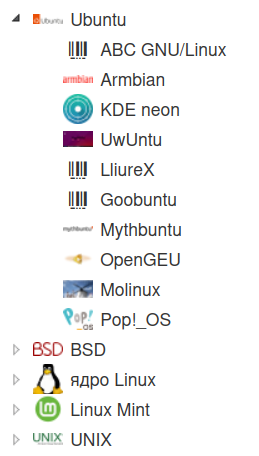
\includegraphics[width=3cm]{chapter/operating_system/base-os-ubuntu.png}
    \caption{Дерево операционных систем, при этом <<вложенные>> системы основаны на базовых системах, размещённых на верхнем уровне дерева}
	\label{fig:base-os-ubuntu}%
\end{marginfigure}

\begin{enumerate}
	\item Вывести список операционных систем с информацией о разработчиках. Ответ на с.~\pageref{answer:os_and_developers}.
	\item Вывести список операционных систем с их логотипами. Ответ на с.~\pageref{answer:os_and_logos}.
	\item Найти страны происхождения операционных систем. Ответ на с.~\pageref{answer:os_country}.
    \item Создать запрос, создающий диаграмму в виде дерева (рис.~\ref{fig:count-software-written-on-languages}). 
        Строчки верхнего уровня должны содержать операционные системы. 
        При <<разворачивании>> мы должны видеть список операционных систем, 
        которые основывались на системе из строчки верхнего уровня. 
        Ответ на с.~\pageref{answer:os_and_bases}.
\end{enumerate}
